\chapter{Theory}
\label{theory}

This thesis presents two new analyses of the prospects for measuring the $H\rightarrow WW$ branching ratio and the forward-backward asymmetry in \ttbar production at CLIC during the 1.4~TeV operational stage. It is therefore important to understand the physics behind these measurements and examine their significance in the context of the physics programme of both CLIC and the wider state of particle physics.


\section{The Standard Model}

The \ac{SM} is a quantum field theory representing our current description of fundamental particles and the interactions between them. It consists of twelve spin-$\frac{1}{2}$ fermions (and their corresponding antiparticles), five spin 1 gauge bosons and one spin 0 scalar boson (as shown in \reffig{tab:smparticles}) where the interactions of the model are described by an $SU(3)_{C}\oplus SU(2)_{L}\oplus SU(1)_{Y}$ local gauge symmetry. The model describes point like particles which interact via the strong, weak and electromagnetic forces. No gravitational interactions are described within the model.

\begin{table}
  \centering
  \begin{tabular}{l c c c c}
    \toprule
    Type  & Name & Mass & Charge (e) & Spin  \\
    \midrule
    Quark & Up & 2.2$^{+ 0.6}_{-0.4}$ MeV & +2/3 & 1/2 \\
    Quark & Down & 4.7$^{+ 0.5}_{-0.4}$ MeV &  -1/3 & 1/2 \\
    \midrule
    Quark & Charm & 1.28$^{+ 0.3}_{-0.3}$ GeV& +2/3 & 1/2 \\
    Quark & Strange & 96$^{+ 8}_{-4}$ MeV& -1/3 & 1/2 \\
    \midrule
    Quark & Top & 173.4$^{+ 1.1}_{-1.1}$ GeV & +2/3 & 1/2 \\
    Quark & Bottom & 4.18$^{+ 0.04}_{-0.03}$ GeV& +1/3 & 1/2 \\
    \midrule
    \midrule
    Lepton & Electron & 0.5109989461$\pm$0.0000000031 MeV & -1 & 1/2 \\
    Lepton & Muon & 105.6583745$\pm$0.0000024 MeV& -1 & 1/2 \\
    Lepton & Tau & 1776.86$\pm$0.12 MeV & -1 & 1/2 \\
    \midrule
    Lepton & Electron Neutrino & $<$2 eV & 0 & 1/2 \\
    Lepton & Muon Neutrino & $<$2 eV & 0 & 1/2 \\
    Lepton & Tau Neutrino & $<$2 eV & 0 & 1/2 \\
    \midrule
    \midrule
    Gauge Boson & W$^+$ & 80.385$\pm$0.015 GeV& 1 & 1 \\
    Gauge Boson & Z & 91.1876$\pm$0.0021 GeV & 0 & 1 \\
    Gauge Boson & $\gamma$ & 0 & 0 & 1 \\
    Gauge Boson & gluon & 0 & 0 & 1 \\
    \midrule
    \midrule
    Scalar Boson & Higgs & 125.09$\pm$0.24 GeV & 0 & 0 \\
    \bottomrule
  \end{tabular}
  \caption[Particles of the Standard Model]{Particles of the Standard Model \cite{Patrignani:2016xqp}}
  \label{tab:smparticles}
\end{table}

The fermions of the model can be classified into two families, leptons and quarks, according to how they interact. The quark family consists of the up(u), down(d), charm(c), strange(s), top(t) and bottom(b) quarks, all of which are capable of interacting via the strong, weak and electromagnetic forces. The lepton family, consisting of the electron(e), muon($\mu$), tau($\tau$), electron neutrino($\nu_{e}$), muon neutrino($\nu_{\mu}$) and tau neutrino($\nu_{tau}$), are defined by the fact they carry no color charge and so are incapable of interacting via the strong force, however they all interact via the weak force and the $e$/$\mu$/$\tau$ can interact electromagnetically. The gauge bosons are the mediators of the three fundamental forces of the model. The photon is a massless boson that mediates the electromagnetic force by coupling to particles with electrical charge. The gluon is also massless and mediates the strong force by coupling to particles with color charge. The gluon is unique amongst the gauge bosons in that it is the only boson that carries the charge to which it couples (i.e. it is colored) and so couples to itself. One direct consequence of this is that it is impossible to form a stable colored state due to color confinement and so quarks are only observed in net-colorless states called hadrons. When a quark is produced in an interaction, it will typically undergo a process known as hadronization in which the quark will bind to quarks/antiquarks spontaneously produced from the vacuum to form quark-antiquark pairs known as mesons, or triplets of quarks or antiquarks known as baryons. The only exception to this is the top quark which will typically decay on a far shorter timescale than is needed for hadronization to occur. The final three gauge bosons are the Z, W$^+$ and W$^-$ which are all massive and mediate the weak interaction via their coupling to weak isospin.

Much like the fermions can be separated into quarks and leptons according to the way they interact, the underlying symmetry of the \ac{SM} of $SU(3)_{C}\oplus SU(2)_{L}\oplus SU(1)_{Y}$ can be decomposed into separate parts according to the interactions that the symmetries describe. The $SU(3)_{C}$ group represents transformations of the color state of a system and so describes interactions involving the strong force. These interactions are commonly referred to as \ac{QCD}. The $SU(2)_{L}\oplus SU(1)_{Y}$ symmetry represents electroweak theory- a unified description of the weak and electromagnetic interactions. In this description, fermions can be thought of as consisting of left and right handed fields, where the left handed components transform as doublets under SU(2) transformations while the right handed components only transform as singlets. The result of this is that the weak interaction only acts on the left handed field components. Hence the weak force only couples to left(right) handed particles (antiparticles.) 

One of the most interesting features of electroweak theory occurs when considering the effect of gauge transformations on the Lagrangian of the system. In quantum field theory, fermions can be described by a Dirac field with the following Lagrangian\cite{Pich:2005mk}

\begin{equation}
  \label{eq:diracLagrangian}
\mathscr{L}=i\bar{\psi}(x) \gamma^{\mu} \partial{_\mu} \psi(x)  -m\bar{\psi}(x)\psi(x),
\end{equation}

Applying a global phase transition of the form

\begin{equation}
\psi(x) \rightarrow \psi '(x) = e^{iQ\alpha}\psi(x),
\end{equation}

will leave the Lagrangian unchanged due to the fact $e^{i\alpha}\psi e^{-i\alpha}\psi=1$. However, in the case of local gauge transformations we replace the global phase transformation by a local one i.e. $\alpha \rightarrow\alpha(x) $ i.e. the phase has a local space-time dependence, then \refeq{eq:diracLagrangian} is no longer invariant as

\begin{equation}
  \partial{_\mu} \psi(x)\rightarrow e^{iQ\alpha(x)} (\partial{_\mu} + iQ\partial{_\mu}\alpha(x)) \psi(x).
\end{equation}

In order to restore the invariance, the derivative $\partial{\mu}$ must be replaced with the covariant derivative $D_{\mu}$ which is of the form

\begin{equation}
  D_{\mu}=\partial{_\mu}+ieA_{\mu},
\end{equation}

where $A_{\mu}$ is a gauge field which transforms as

\begin{equation}
  A_{\mu}\rightarrow A_{\mu}^{'} = A_{\mu} - \frac{1}{e}\partial{_\mu}\alpha(\textbf{x}).
\end{equation}

In electroweak theory the gauge fields required are found to consist of three weak isospin fields, $W_1, W_2$ and $W_3$,  coming from the SU(2) group and one weak hypercharge field, B, from U(1). The interesting result of this is the prediction that the bosons associated with these fields and the fermions they interact with should be massless. However, this is not supported by data as the bosons of the weak force, Z and W, have masses of $m_Z$=91.876 $\pm$ 0.0021 GeV and $m_W$=80.385 $\pm$ 0.015 GeV respectively\cite{Patrignani:2016xqp}. Furthermore, in electroweak theory it can be shown that the presence of massive electroweak bosons results in unphysical predictions in the \ac{SM} e.g. violation of unitarity when calculating the amplitude of $WW\rightarrow WW$ scattering \cite{Szleper:2014xxa}. These problems can be fixed via consideration of the final particle within the \ac{SM}, the Higgs boson.

\section{The Higgs Boson and the Origin of Mass}

To solve the problems seen in the electroweak sector, Brout, Englert and Higgs \cite{PhysRevLett.13.508}\cite{PhysRevLett.13.321} proposed that mass terms could be generated within the \ac{SM} via the addition of a complex, scalar doublet of the group $SU(2)$ possessing four degrees of freedom

\begin{equation}
\phi = \begin{pmatrix} \phi^{+} \\ \phi^{0} \end{pmatrix}, 
\end{equation}

with potential

\begin{equation}
V(\phi) = \mu^{2}\phi^{\dagger}\phi + \frac{\lambda^{2}}{2}(\phi^{\dagger}\phi)^{2},
\end{equation}

where $\mu^{2}$ is the negative mass squared parameter and $\lambda$ is the Higgs field self-coupling.

The Higgs field is found to interact with the $W_{1},W_{2},W_{3}$ and $B$ gauge fields. In the case that $\mu^{2}<0$, due to the Higgs field acquiring a non-zero expectation value, the $SU(2)_{L}\oplus SU(1)_{Y}$ symmetry is found to break leaving only a $U(1)_{em}$ symmetry corresponding to a massless photon. Of the four degrees of freedom associated with the Higgs field, the interaction of the field with the W and B gauge fields results in three massive gauge bosons corresponding to the measured $Z$ and $W^{\pm}$ masses, where the physically observed bosons actually represent mixtures of the underlying gauge fields

\begin{equation}
\gamma = \cos\theta_{W}B  +\sin\theta_{W}W_{3}, 
\end{equation}

\begin{equation}
Z = \cos\theta_{W}W_{3}  -\sin\theta_{W}B,
\end{equation}

\begin{equation}
W^{\pm}= \frac{1}{\sqrt{2}}(W_{1}\mp iW_{2}),
\end{equation}

and where $\theta_{W}$ is the weak mixing angle.

The last remaining degree of freedom of the Higgs field corresponds to the Higgs boson itself. The mass of the Higgs boson can be determined to be $m_{H}=\sqrt{2\lambda}\nu$, where $\nu$ is the vacuum expectation value for the Higgs field. While $\nu$ can be calculated within the standard model, $\lambda$ is a free parameter and so the mass of the Higgs is not known a priori. Experimentally it is found to be $\sim$125GeV\cite{:2012gk,Chatrchyan:2012xdj}.

While the mass of the Higgs is of special interest because its value is a free parameter in the standard model, there are many more properties of the Higgs that are important to measure. In particular, the way in which the Higgs boson couples to other particles is predicted without ambiguity within the \ac{SM} and is expected to vary between various \ac{BSM} models. Within the \ac{SM} the coupling of the Higgs to fermions and bosons varies according to their masses


\begin{equation}
g_{Hf\bar{f}}=\frac{M_f}{\nu} ~~~~~~~~    g_{HBB}=\frac{2M_B^2}{\nu} .
\end{equation}

Therefore, characterizing the coupling to each fermion as a function of the fermions mass represents a powerful way of testing the \ac{SM}. The mass dependence on the Higgs couplings also presents a new way to perform indirect searches for new physics involving as yet unseen massive particles by looking at the branching ratio of Higgs decays to invisible decay products and the total Higgs decay width. This is of particular interest in searches for dark matter which is known to interact gravitationally and so must possess mass. 

\section{Higgs Measurements at CLIC}
\begin{figure}
  \centering
  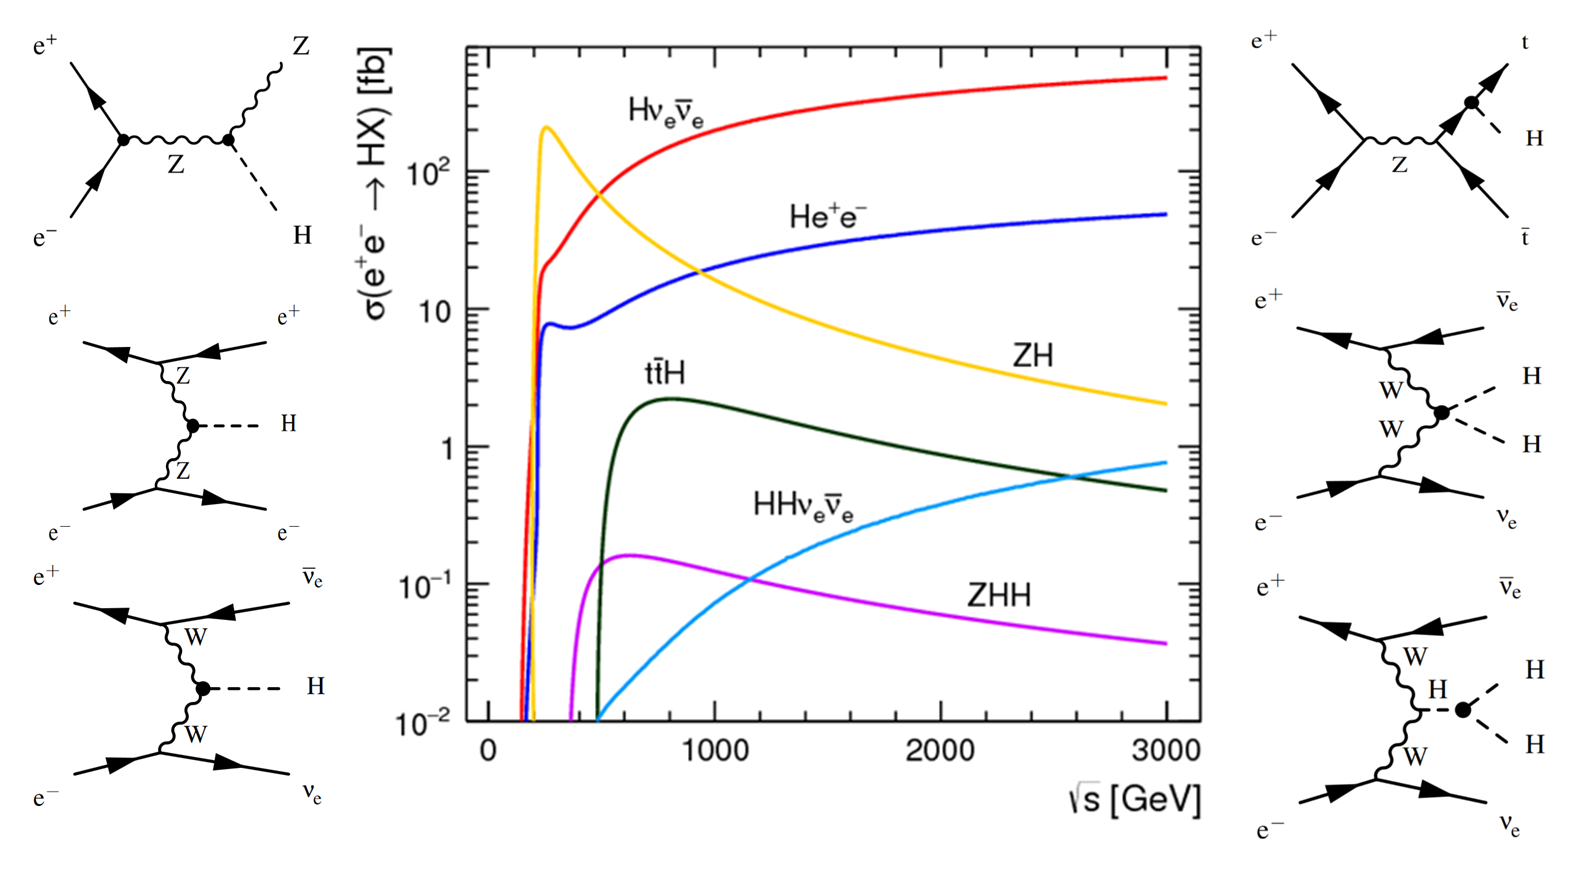
\includegraphics[width=0.95\textwidth,keepaspectratio]{Theory/fig/HiggsProcessesExtra.png}
  \caption[Cross sections for Higgs production mechanisms]{Cross sections for Higgs production mechanisms \cite{Abramowicz:2016zbo}.}
  \label{fig:higgsXSecs}
\end{figure}

The CLIC physics programme places substantial emphasis on characterizing the Higgs boson as it presents a new and relatively less well measured sector of the \ac{SM} to explore. In particular it will aim to measure the mass, width, and couplings of the Higgs in a model independent manner. Electron positron collisions provide access to numerous Higgs production mechanisms which can be seen in \reffig{fig:higgsXSecs}. Due to the strong energy dependence on many of the cross sections on energy, different processes will be of interest at each of the three energy stages operated at CLIC. At 380GeV the focus will predominantly be on measuring the Higgsstrahlung ($ZH$) process in which a Z boson radiates a Higgs, while at higher energies vector boson fusion ($H\nu\bar{\nu},He^{+}e^{-}$) dominates and new processes such as di-Higgs production become accessible. A summary of all the results from current Higgs studies performed by CLIC is available in \cite{Abramowicz:2016zbo}.

\subsection{Higgsstrahlung}

\begin{figure}
  \centering
  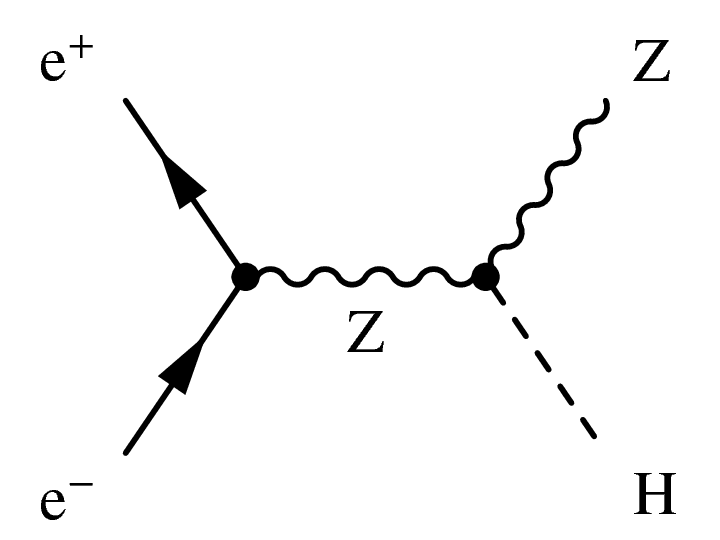
\includegraphics[width=0.45\textwidth,keepaspectratio]{Theory/fig/HiggsStrahlung.png}
  \caption[The Higgstrahlung Process]{The Higgstrahlung Process.}
  \label{fig:higgsstrahlung}
\end{figure}


One of the key aims of the experiment will be to examine the Higgsstrahlung process shown in \reffig{fig:higgsstrahlung}. In this process, if the four-momentum of the Z boson can be measured to high precision, then because the initial conditions of the collision are well known, one can determine the mass of the particle it is recoiling against ($m_{rec}^{2} = s + m_{z}^{2} - 2E_{z}\sqrt{s}$, with $E_Z$ being the measured energy of the Z) and infer the presence of a Higgs boson on an event-by-event basis. This allows properties such as the Higgs mass, cross-section and coupling to the Z to be measured without actually using the decay products of the Higgs boson directly, which in turn allows the measurements to be model independent. This method is not possible at hadron colliders such as the LHC where, even though the Higgsstrahlung process still occurs, the four momentum of the colliding particles can never be known as precisely due to their composite nature. Using the clean signal from cases where the Z decays to a pair of muons or electrons it is possible to measure the recoil mass to high precision and thus determine the mass of the Higgs to $\Delta m_{H} = 110$~MeV (see \reffig{fig:higgsmass}) using data from the low energy stage only. This value can be further improved to $\Delta m_{H} = 44~MeV$ when including direct measurement results from the $ee\rightarrow H\nu\bar{\nu}, H\rightarrow b\bar{b}$ channel at 3~TeV. Despite giving a poorer resolution on the Z four momentum, the $Z\rightarrow qq$ higgsstrahlung channel is also considered due to its larger cross section. Using this channel a limit of $BR(H\rightarrow invis.) <0.97\%$ at 90\% C.L. can be set. 

\begin{figure}
  \centering
  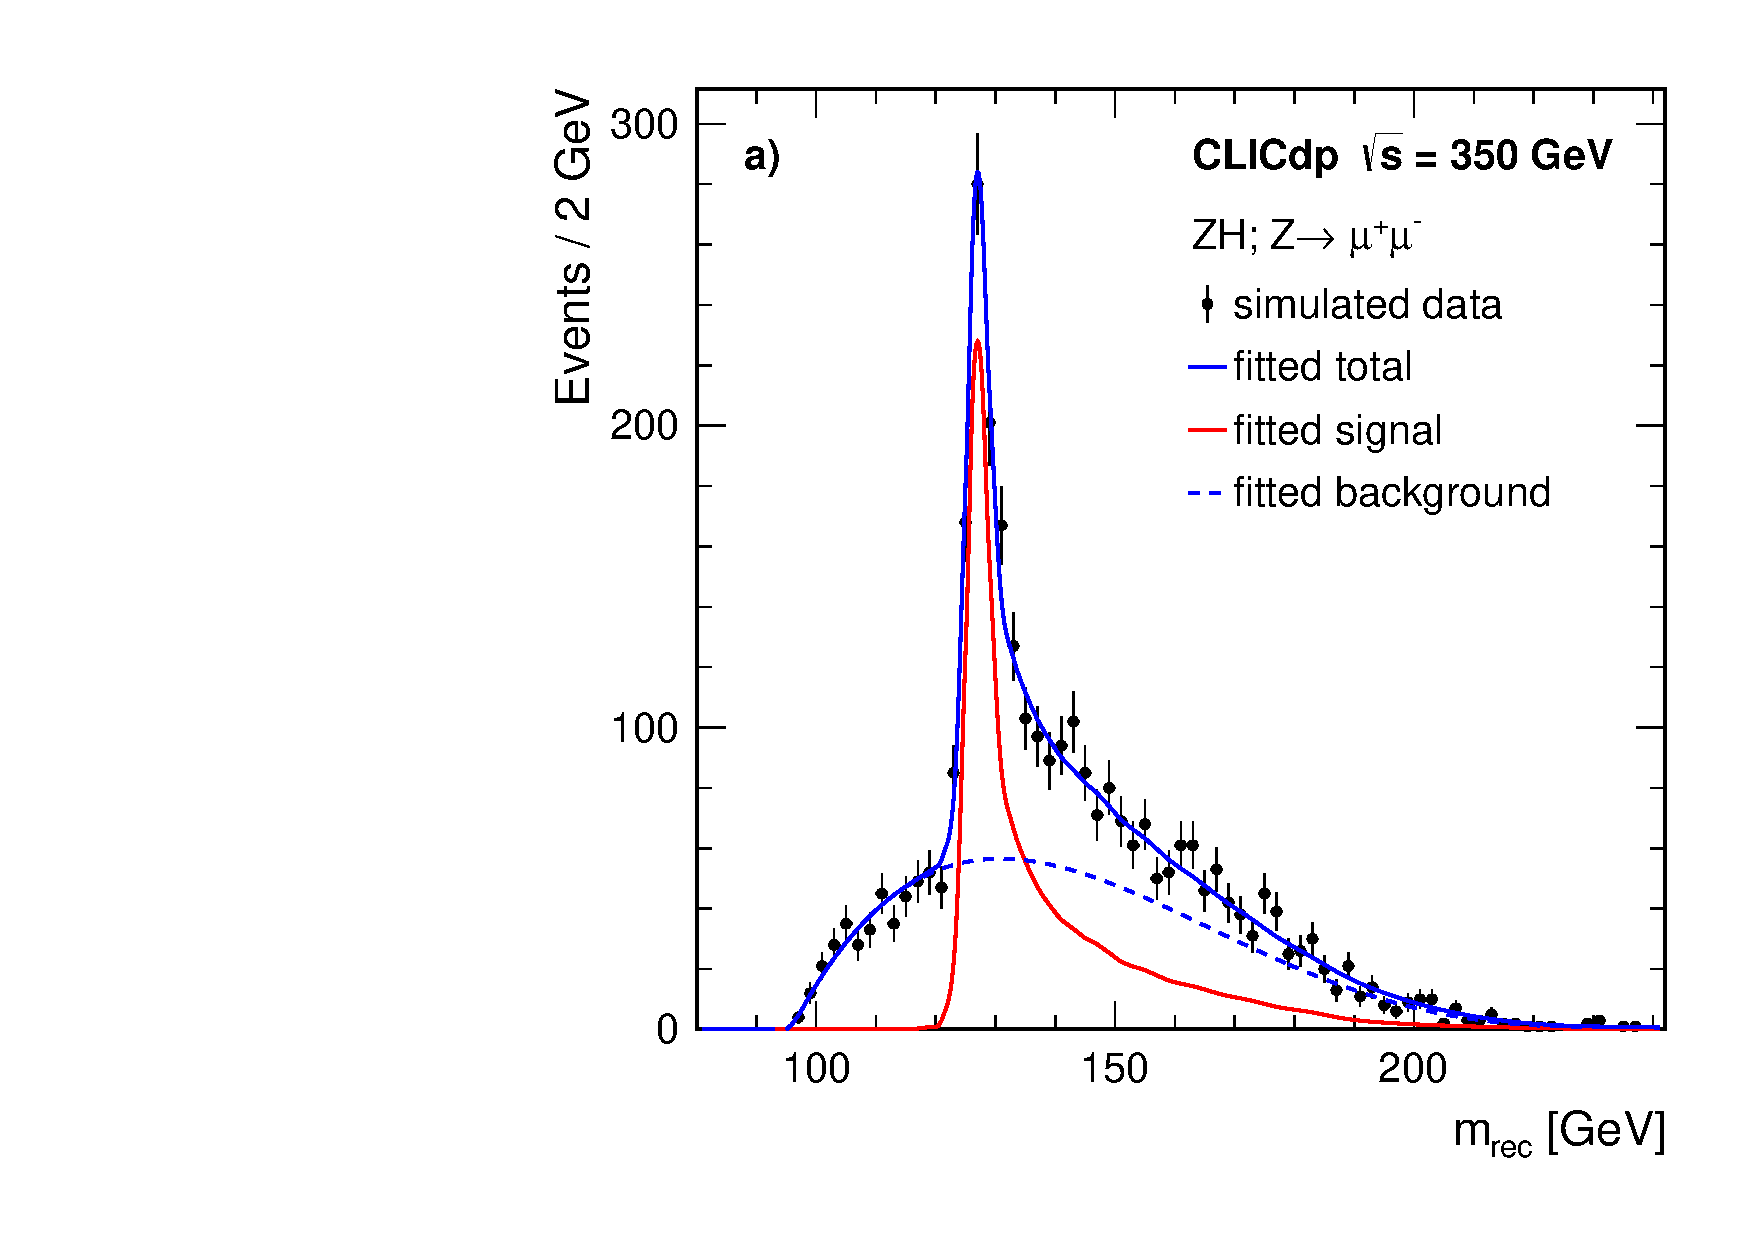
\includegraphics[width=0.45\textwidth,keepaspectratio]{Theory/fig/350GeV_Recoil_mumuX_MrecoilFit.pdf}
  \caption[Reconstructed recoil mass from Higgsstralung process]{Reconstructed recoil mass from Higgsstralung process \cite{Abramowicz:2016zbo}.}
  \label{fig:higgsmass}
\end{figure}

 
\subsection{Model Independent Extraction of Higgs Couplings}


While the Higgsstrahlung alone allows the mass and branching ratios of the Higgs to be determined, it is further possible to extract the absolute width of the Higgs, $\Gamma_H$, by measuring the rates of several different Higgs processes and combining them in the right ratio. One such scheme proposed for doing this is shown in \refeq{modelindependentformula} \cite{Durig:2014lfa}

\begin{equation}
  \label{modelindependentformula}
  \Gamma_H = \frac{X_1^2X_3^2}{X_4^2X_2},
\end{equation}

where

\begin{equation}
X_1=\sigma_{ZH} \propto g_{HZZ}^2
\end{equation}

\begin{equation}
  \label{X2}
  X_2=\sigma_{H\nu\bar{\nu}} \times BR(H\rightarrow WW^*) \propto \frac{g_{HWW}^4}{\Gamma_H}
\end{equation}

\begin{equation}
X_3=\sigma_{H\nu\bar{\nu}} \times BR(H\rightarrow b\bar{b}) \propto \frac{g_{HWW}^{2}g_{Hbb}^2}{\Gamma_H}
\end{equation}

\begin{equation}
X_4=\sigma_{ZH} \times BR(H\rightarrow b\bar{b}) \propto \frac{g_{HZZ}^{2}g_{Hbb}^2}{\Gamma_H}
\end{equation}

 With the exception of $X_1$, the choice of variables used is not unique (e.g. one could replace the production mechanism in $X_1$ and $X_2$ with ZZ-fusion rather than WW-fusion,) however the combination shown here is expected to give the highest precision on $\Gamma_H$ due to the large cross-section associated with WW-fusion and the high branching ratio of $H\rightarrow b\bar{b}$ ($\sim$ 65\%). In chapter \ref{Higgs Analysis} we will present our research on the precision with which $X_2$ can be measured during the 1.4~TeV run at CLIC. Currently at the LHC the standard process for extracting couplings from the equivalent measurements of $X_{2,3\&4}$ is to multiply through by the standard model value of the Higgs width \cite{ATLAS-CONF-2015-044}. This type of measurement is referred to as ``model-dependent'' as the values determined for the Higgs couplings implicitly assume the \ac{SM} Higgs width. At CLIC, because the width can be measured experimentally there is no need to make this assumption and so the couplings are measured in a ``model-independent'' way. The unique ability of $e^+e^-$ colliders to perform model-independent measurements is one of the largest driving factors for constructing and using them as a so called ``Higgs-Factory''. One limiting factor for the model-independent measurements of the couplings is that they are always ultimately dependent on the precision with which the ZH cross section can be measured (predicted to be $\Delta h_{HZZ} = 0.8\%$\cite{Abramowicz:2016zbo}) as this quantity is always needed in the ratio used to extract $\Gamma_H$.

\begin{table}
  \centering
  \begin{tabular}{lllc}\toprule
     &                                                           &                              & Statistical precision                        \\\cmidrule(l){4-4}
     Channel  & Measurement                                        & Observable            & $350\,\GeV$       \\ 
     &                                                           &                              & $500\,fb^{-1}$        \\ \midrule
     $ZH$            & Recoil mass distribution                                  & $\mH$                        & $110\,\MeV$  \\
     $ZH$            & $\sigma(ZH)\times BR(H\rightarrow \text{invisible})$         & $\Gamma_\text{inv}$          & $0.6\,\%$  \\ \midrule
     $ZH$            & $\sigma(ZH)\times BR(Z\rightarrow l^+l^-)$             & $g^{2}_{HZZ}$                  & $3.8\,\%$  \\
     $ZH$            & $\sigma(ZH)\times BR(Z\rightarrow q\bar{q})$                  & $g^{2}_{HZZ}$                  & $1.8\,\%$  \\
     $ZH$            & $\sigma(ZH)\times BR(H\rightarrow b\bar{b})$                & $g^{2}_{HZZ}g^{2}_{Hbb}/\Gamma_H$     & $0.86\,\%$ \\
     $ZH$            & $\sigma(ZH)\times BR(H\rightarrow c\bar{c})$                & $g^{2}_{HZZ}g^{2}_{Hcc}/\Gamma_H$       & $14\,\%$ \\
     $ZH$            & $\sigma(ZH)\times BR(H\rightarrow gg)$                   &                              & $6.1\,\%$ \\
     $ZH$            & $\sigma(ZH)\times BR(H\rightarrow \tau^+\tau^-)$               & $g^{2}_{HZZ}g^{2}_{H\tau\tau}/\Gamma_H$ & $6.2\,\%$ \\
     $ZH$            & $\sigma(ZH)\times BR(H\rightarrow WW^*)$                 & $g^{2}_{HZZ}g^{2}_{HWW}/\Gamma_H$     & $5.1\,\%$ \\
     $H\nu_e\bar{\nu_e}$    & $\sigma(H\nu_e\bar{\nu_e})\times BR(H\rightarrow b\bar{b})$        & $g^{2}_{HWW}g^{2}_{Hbb}/\Gamma_H$     & $1.9\,\%$ \\
     $H\nu_e\bar{\nu_e}$    & $\sigma(H\nu_e\bar{\nu_e})\times BR(H\rightarrow c\bar{c})$        & $g^{2}_{HWW}g^{2}_{Hcc}/\Gamma_H$     & $26\,\%$ \\
     $H\nu_e\bar{\nu_e}$    & $\sigma(H\nu_e\bar{\nu_e})\times BR(H\rightarrow gg)$        &     & $10\,\%$ \\    
     \bottomrule
   \end{tabular}
   \caption[Expected statistical uncertainties for Higgs measurements at 350~GeV at CLIC assuming unpolarised beams]{Expected statistical uncertainties for Higgs measurements at 350~GeV at CLIC assuming unpolarised beams \cite{Abramowicz:2016zbo}.}
   \label{fig:350GeVNumbers}
\end{table}

\begin{table}
  \centering
  \begin{tabular}{lllcc}\toprule
    &                                                           &                              & Statistical precision                       \\\cmidrule(l){4-5}
    Channel  & Measurement                                        & Observable & $1.4\,\TeV$         & $3\,\TeV$           \\ 
    &                                                           &                           & $1.5\,ab^{-1}$      & $2.0\,ab^{-1}$        \\ \midrule
    $H\nu_e\bar{\nu_e}$    & $H\rightarrow b\bar{b}$ mass distribution                       & $m_H$                & $47\,\MeV$     & $44\,\MeV$       \\ \midrule
    $H\nu_e\bar{\nu_e}$    & $\sigma(H\nu_e\bar{\nu_e})\times BR(H\rightarrow b\bar{b})$        & $g^{2}_{HWW}g_{Hbb}^{2}/\Gamma_H$   & $0.4\,\%$         & $0.3\,\%$           \\
    $H\nu_e\bar{\nu_e}$    & $\sigma(H\nu_e\bar{\nu_e})\times BR(H\rightarrow c\bar{c})$        & $g^{2}_{HWW}g_{Hcc}^{2}/\Gamma_H$  & $6.1\,\%$         & $6.9\,\%$           \\
    $H\nu_e\bar{\nu_e}$    & $\sigma(H\nu_e\bar{\nu_e})\times BR(H\rightarrow gg)$           &                     & $5.0\,\%$         & $4.3\,\%$           \\
    $H\nu_e\bar{\nu_e}$    & $\sigma(H\nu_e\bar{\nu_e})\times BR(H\rightarrow \tau^+\tau^-)$       & $g^{2}_{HWW}g_{H\tau\tau}^{2}/\Gamma_H$ & $4.2\,\%$         & $4.4\,\%$               \\
    $H\nu_e\bar{\nu_e}$    & $\sigma(H\nu_e\bar{\nu_e})\times BR(H\rightarrow \mu^+\mu^-)$       & $g^{2}_{HWW}g_{H\mu\mu}^{2}/\Gamma_H$   & $38\,\%$        & $25\,\%$            \\
    $H\nu_e\bar{\nu_e}$    & $\sigma(H\nu_e\bar{\nu_e})\times BR(H\rightarrow \gamma\gamma)$ &                          & $15\,\%$          & $10\,\%^*$               \\
    $H\nu_e\bar{\nu_e}$    & $\sigma(H\nu_e\bar{\nu_e})\times BR(H\rightarrow Z\gamma)$      &                             & $42\,\%$           & $30\,\%^*$               \\
    $H\nu_e\bar{\nu_e}$    & $\sigma(H\nu_e\bar{\nu_e})\times BR(H\rightarrow WW^*)$         & $g_{HWW}^{4}/\Gamma_H$            & $1.0\,\%$         & $0.7\,\%^*$         \\
    $H\nu_e\bar{\nu_e}$    & $\sigma(H\nu_e\bar{\nu_e})\times BR(H\rightarrow ZZ^*)$         & $g^{2}_{HWW}g_{HZZ}^{2}/\Gamma_H$  & $5.6\,\%$ & $3.9\,\%^*$   \\
    $He^+e^-$       & $\sigma(He^+e^-)\times BR(H\rightarrow b\bar{b)}$           & $g_{HZZ}^{2}g_{Hbb}^{2}/\Gamma_H$    & $1.8\,\%$ & $2.3\,\%^*$ \\ \midrule
    $t\bar{t}H$      & $\sigma(t\bar{t}H)\times BR(H\rightarrow b\bar{b})$          & $g_{Htt}^{2}g_{Hbb}^{2}/\Gamma_H$  & $8\,\%$         & $-$             \\
    $HH\nu_e\bar{\nu_e}$ & $\sigma(HH\nu_e\bar{\nu_e})$                               & $\lambda$                   & $54\,\%$          & $29\,\%$            \\
    $HH\nu_e\bar{\nu_e}$ & with $-80\,\%$ $e^-$ polarisation                             & $\lambda$                  & $40\,\%$          & $22\,\%$            \\ \bottomrule
  \end{tabular}
  \caption[Expected statistical uncertainties for Higgs measurements at 1.4~TeV and 3~TeV at CLIC assuming unpolarised beams]{Expected statistical uncertainties for Higgs measurements at 1.4~TeV and 3~TeV at CLIC assuming unpolarised beams \cite{Abramowicz:2016zbo}. Values marked with a * represent extrapolations from studies performed at 1.4~TeV.}
  \label{fig:HighENumbers}
\end{table}

\begin{figure}
  \centering
  \begin{subfigure}{.49\textwidth}
    \centering
    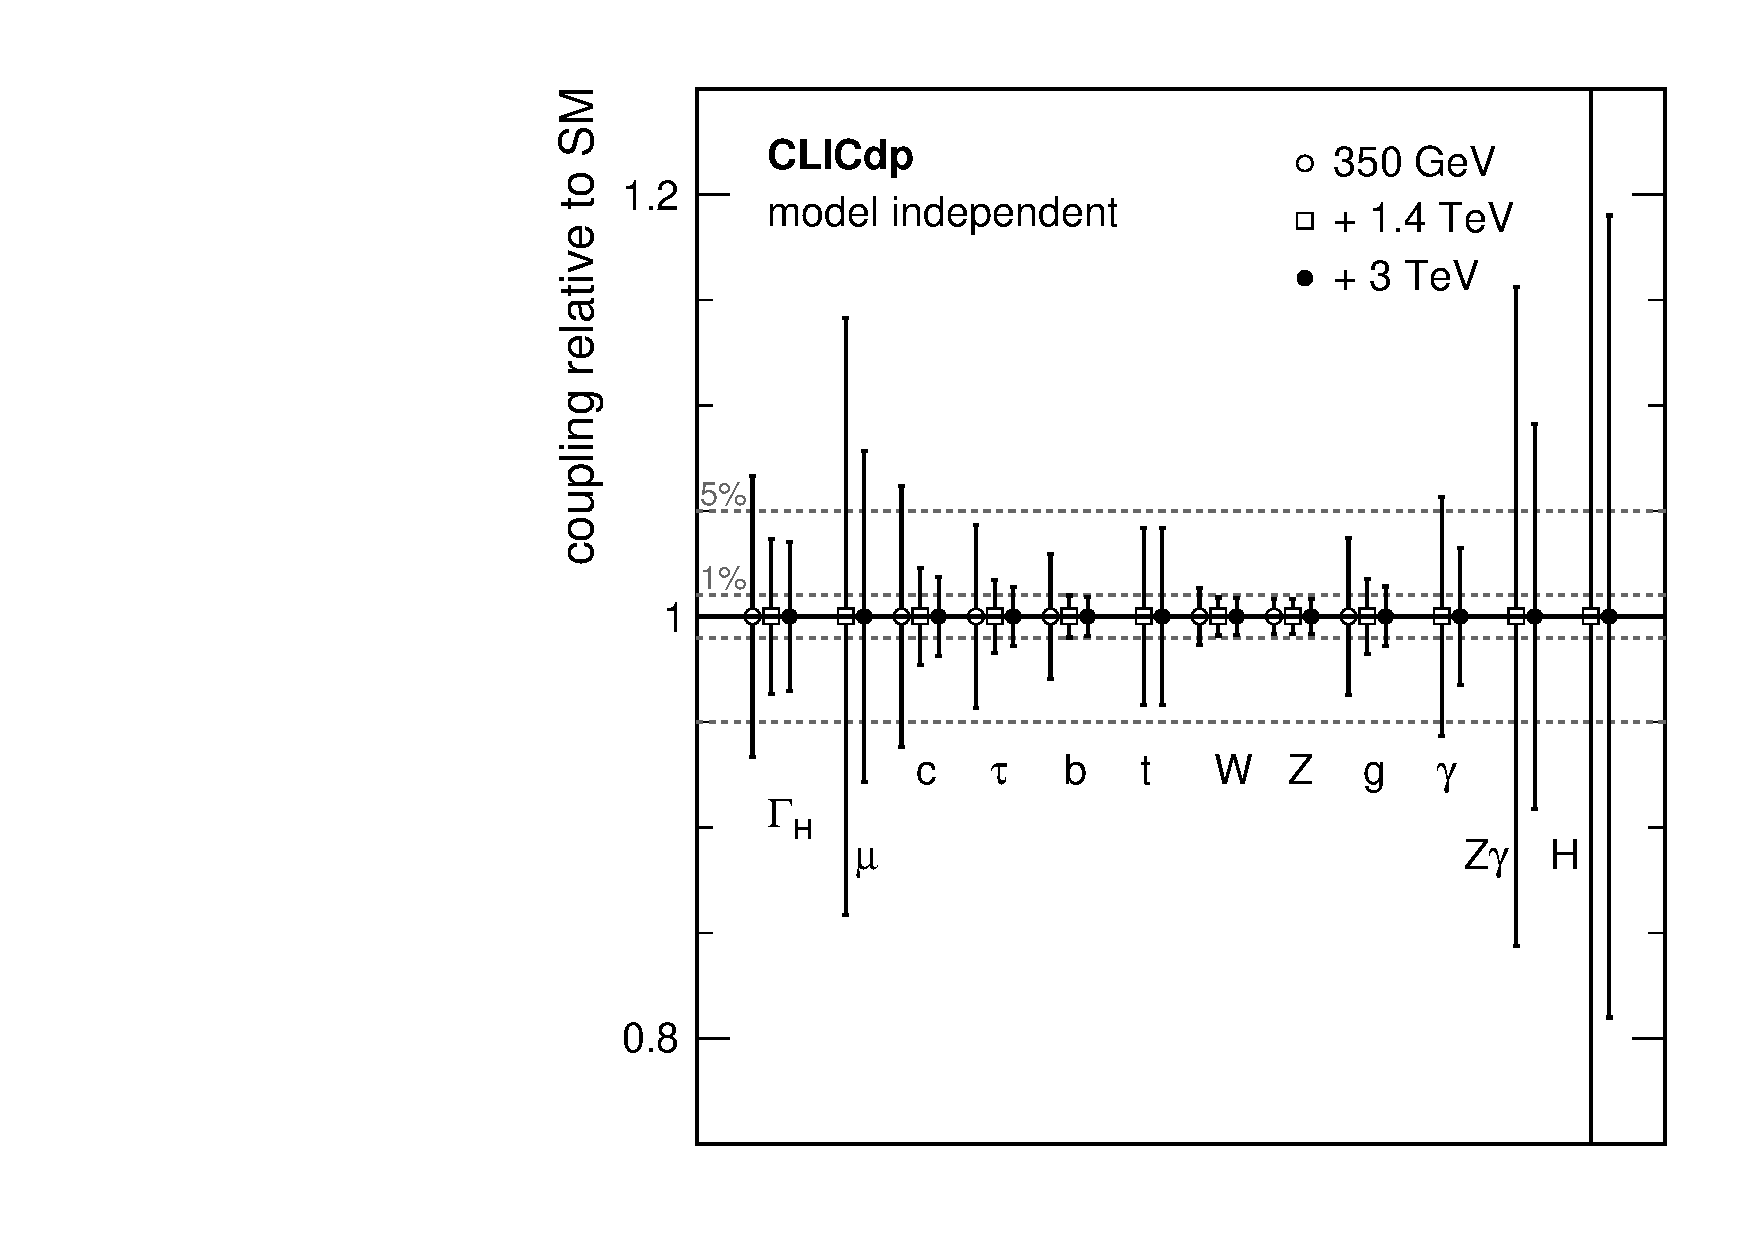
\includegraphics[width=0.95\linewidth]{Theory/fig/FitResultsMI.pdf}
  \end{subfigure}
    \begin{subfigure}{.49\textwidth}
    \centering
    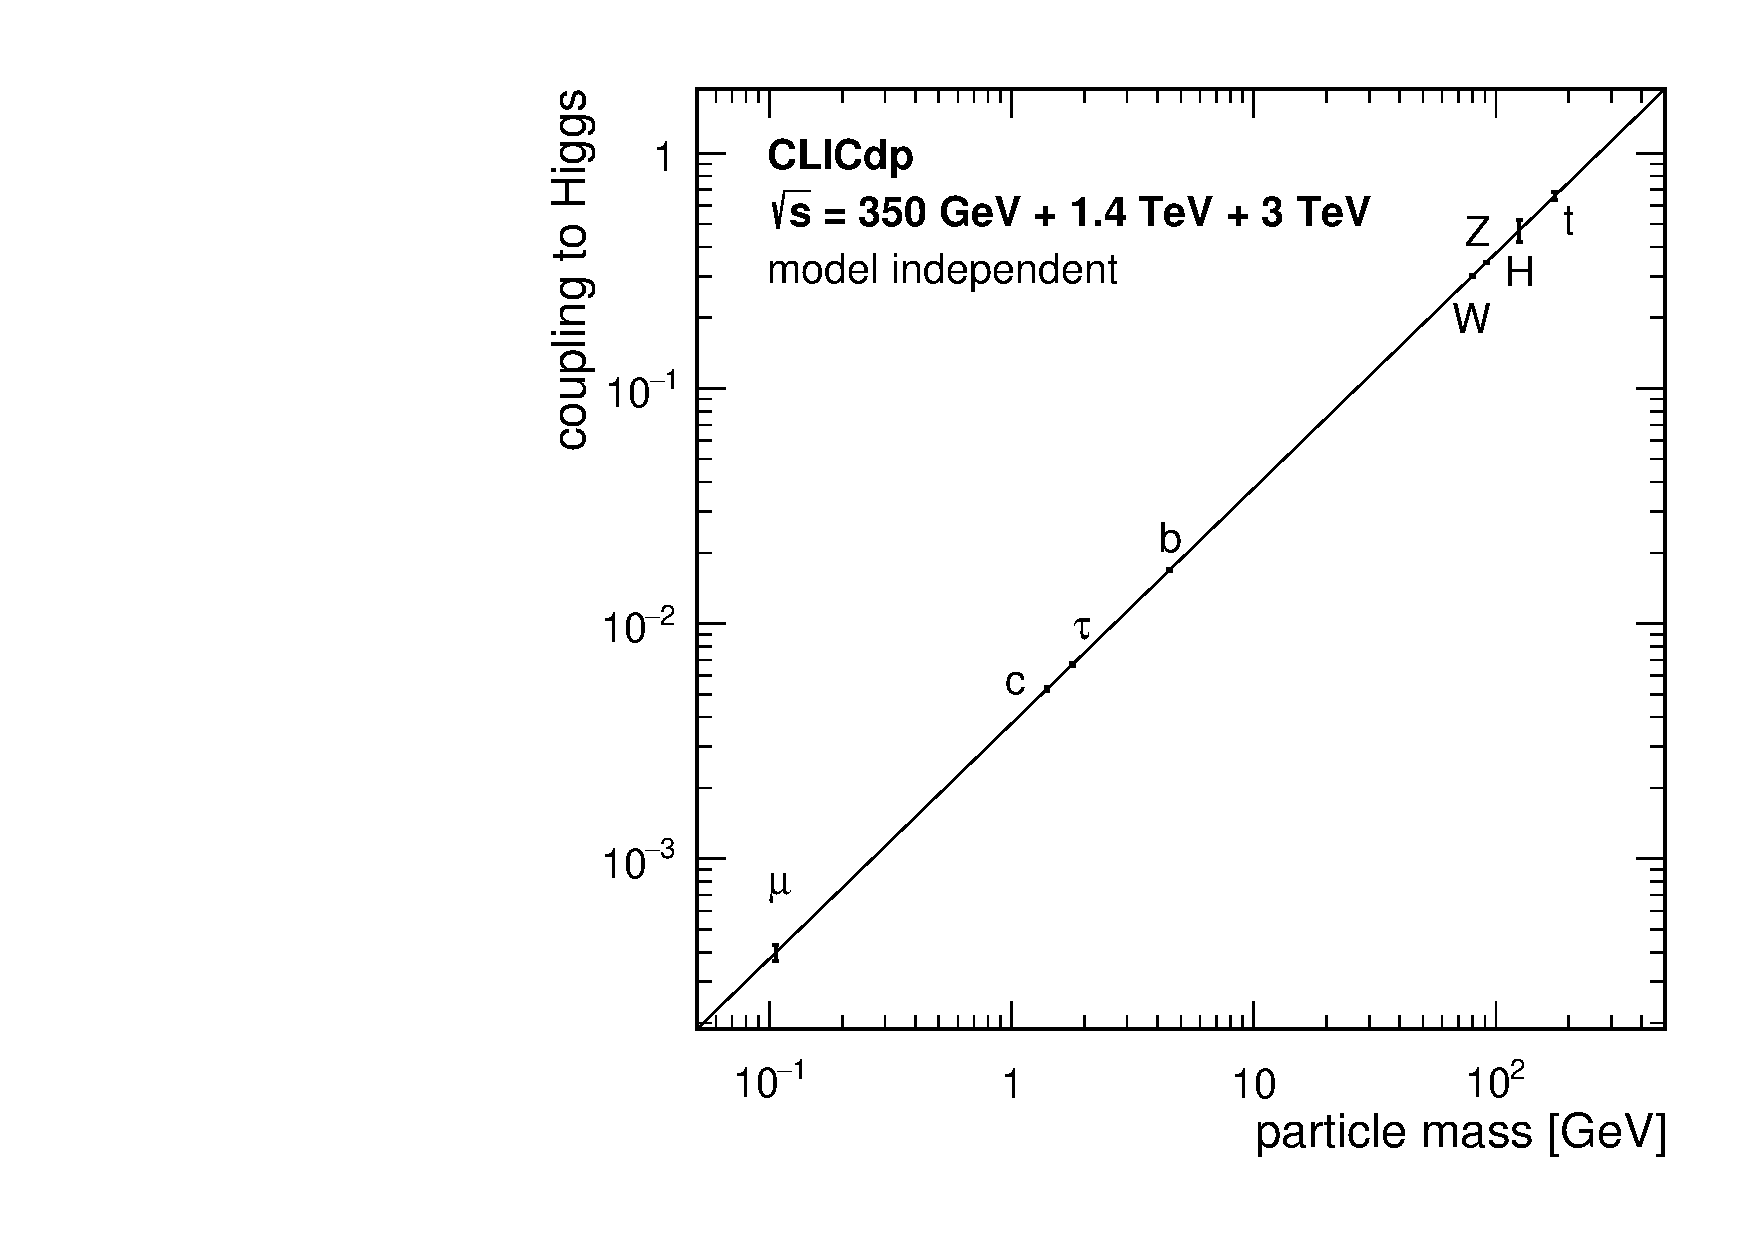
\includegraphics[width=0.95\linewidth]{Theory/fig/CouplingvsMassMI.pdf}
  \end{subfigure}
    \caption[Expected precision on model independent measurements of the Higgs couplings]{Expected precision on model independent measurements of the Higgs couplings \cite{Abramowicz:2016zbo}.}
  \label{fig:modelIndependentCouplings}
\end{figure}

\begin{figure}
\centering
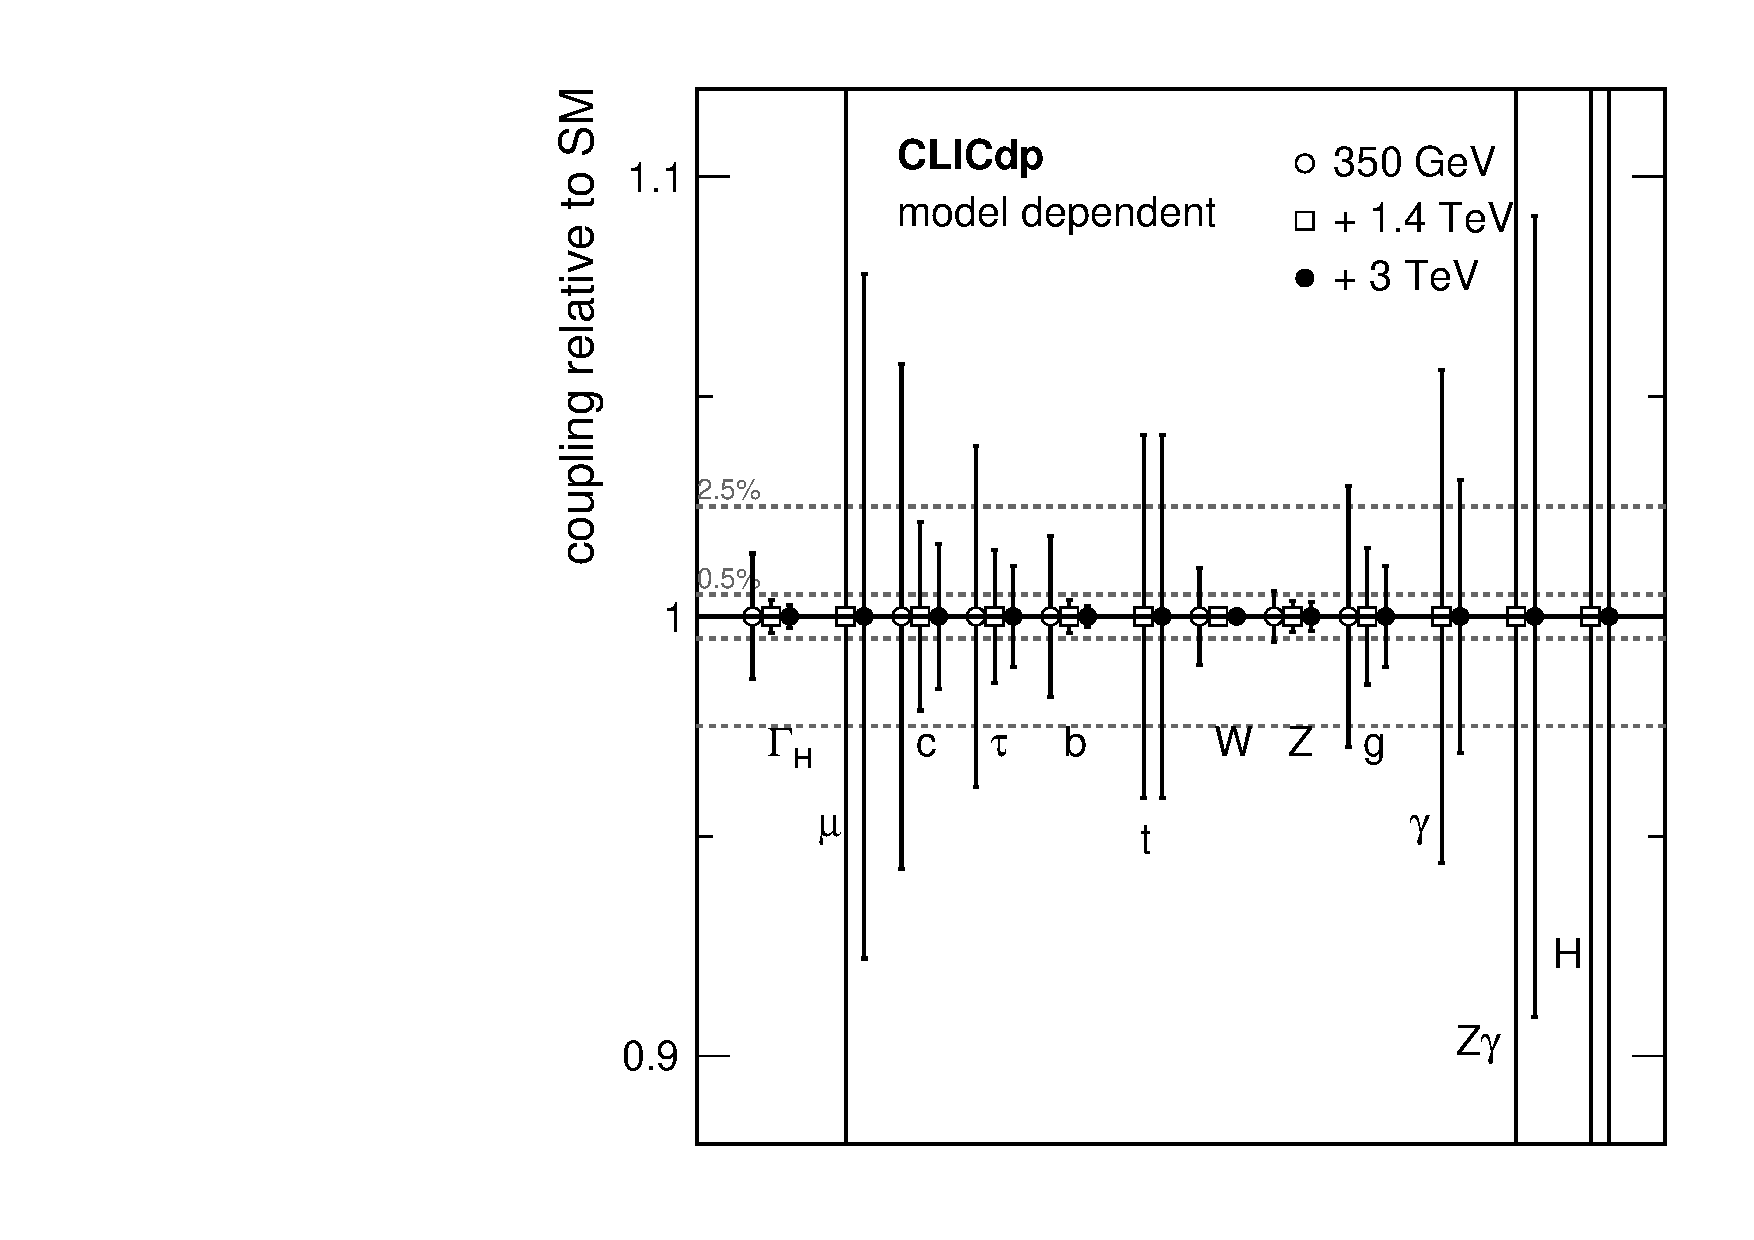
\includegraphics[width=0.65\linewidth]{Theory/fig/FitResultsMD.pdf}
\caption[Expected precision on model dependent measurements of the Higgs couplings at CLIC]{Expected precision on model dependent measurements of the Higgs couplings at CLIC \cite{Abramowicz:2016zbo}.}
\label{fig:modelDependentCouplings}
\end{figure}

\begin{figure}
\centering
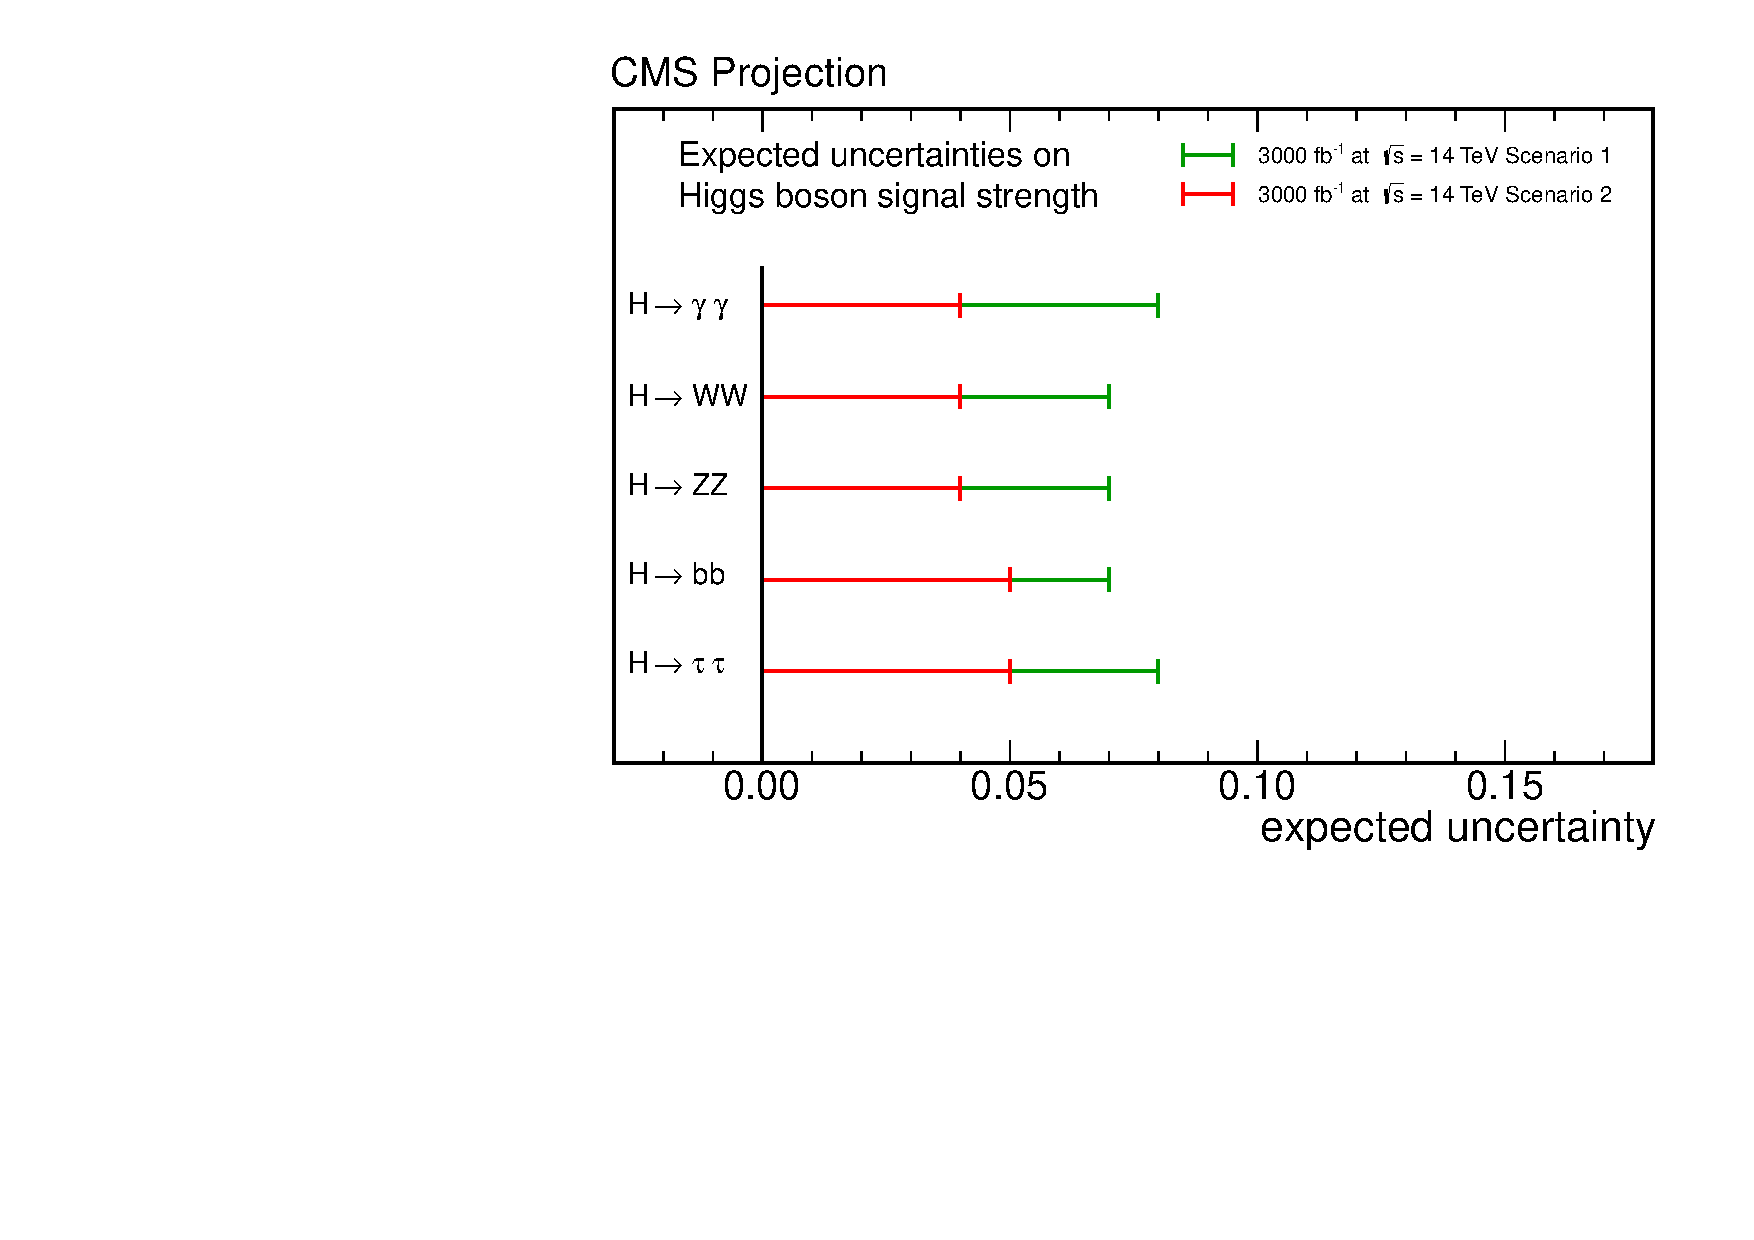
\includegraphics[width=0.7\linewidth]{Theory/fig/MuSnowmass3000.pdf}
\caption[Expected precision on model dependent measurements of the Higgs couplings at CMS]{Expected precision on model dependent measurements of the Higgs couplings at \ac{CMS} for the \ac{HL-LHC}. Scenario 1 represents a case where the systematic and theoretical uncertainties remain at their current levels. In scenario 2 the theoretical uncertainty is scaled by a factor of a half and the systematic uncertainties are scaled by the square root of the integrated luminosity \cite{CMS:2013xfa}.}
\label{fig:CMSHiggsPredictions}
\end{figure}

In practice it is expected that an 11 parameter global fit to multiple variations of these measurements will be performed at each stage of operation to extract the Higgs width and its couplings to both fermions and bosons. The relevant inputs for these fits are shown in \reftab{fig:350GeVNumbers} and \ref{fig:HighENumbers} while the results of the fits are shown in \reffig{fig:modelIndependentCouplings}.

For context it is also important to compare these results to what can be expected from experiments such as ATLAS and CMS at the LHC. Because the Higgs width can not be explicitly calculated at hadron colliders, it is appropriate to compare the model dependent version of the CLIC analysis with those predicted by ATLAS and CMS. In this situation, because the precision of the couplings is no longer limited by the precision on $g_{HZZ}$, the predicted precision for CLIC is seen to improve considerably. One can see from \reffig{fig:modelDependentCouplings} and \ref{fig:CMSHiggsPredictions} that in many cases CLIC is expected to provide an order of magnitude improvement over what can be achieved at the LHC with many of the key parameters associated with the Higgs being measured to sub percent precision.

Ultimately the aim of performing precision measurements is to allow the validation or rejection of theoretical models. While the results seen so far at the LHC suggest that the observed Higgs boson is that of the \ac{SM}, there are numerous alternative theories that predict a Higgs like particle with properties similar to what has been observed but which differ to a degree not yet measurable by current experiments. The details of these theories will not be expanded upon within this thesis, however the deviations expected in the Higgs couplings of these theories relative to the \ac{SM} are shown in \reftab{table:snowmass}. These values should only be taken as a rough guideline for the precision required to discover/reject the theories as they are based on the assumption that new physics occurs at a specific scale (in this case 1~TeV). Although the precision required to provide sensitivity to these models is expected to be greater than that expected for the LHC, it may be within the scope of the proposed CLIC physics programme.  

\begin{table}
  \centering
  \begin{tabular}{l c c c}
    \toprule
    \toprule
    Model  & $\kappa_V$ & $\kappa_b$ & $\kappa_\gamma$  \\
    \midrule
    Singlet Mixing & $\sim$6\% & $\sim$6\%  & $\sim$6\% \\
    2HDM & $\sim$1\% & $\sim$10\%  & $\sim$1\% \\
    Decoupling MSSM & $\sim$-0.0013\% & $\sim$1.6\%  & $\sim$-.4\% \\
    Composite & $\sim$-3\% & $\sim$-(3-9)\%  & $\sim$-9\% \\
    Top Partner & $\sim$-2\% & $\sim$-2\%  & $\sim$+1\% \\
    \bottomrule
    \bottomrule
  \end{tabular}
  \caption[Predicted Higgs Coupling Modifications for BSM theories]{Generic size of Higgs coupling modifications from the \ac{SM} values when all new particles are $M\sim 1 TeV$ and mixing angle satisfy precision electroweak fits. The decoupling MSSM numbers assume $\tan\beta = 3.2$ and a stop mass of 1 TeV with $X_t =0$ for the $\kappa_\gamma$ prediction \cite{Dawson:2013bba}. $\kappa_{V,b,\gamma}$ denote the model dependent couplings of the vector bosons, b quark and photon to the Higgs.}
  \label{table:snowmass}
\end{table}

\section{Top Quark Physics}


The top quark is currently the heaviest particle within the \ac{SM} and is the only quark that decays before undergoing hadronization. Due to its high mass, top interactions are good channels for looking for \ac{BSM} physics with a characteristic energy scale beyond what has currently been discovered. Due to its high mass, the top is also the fermion with the strongest coupling to the Higgs making it a good candidate for finding deviations from the \ac{SM} within the Higgs sector. As such, the physics programme for \ac{CLIC} will measure the top quark's properties during the lowest energy stage of operation featuring a dedicated top threshold scan aiming to provide precision measurements of the top mass and width. The dominant production mechanism for top production is through the $s$-channel: $e^+e^-\rightarrow\gamma /Z\rightarrow t\bar{t}$ process shown in \reffig{fig:topFeynmann}. Using this process the properties of the $t\bar{t}\gamma$ and $t\bar{t}Z$ vertices can be measured. Examining these can provide sensitivity to contributions from \ac{BSM} effects such as the existence of extra bosons (e.g. $Z'$ \cite{Langacker:2008yv}) which could provide an additional production channel, modifying the behavior at the vertex. The  $t\bar{t}X$ vertex can be written as\cite{Amjad:2015mma}

\begin{figure}
\centering
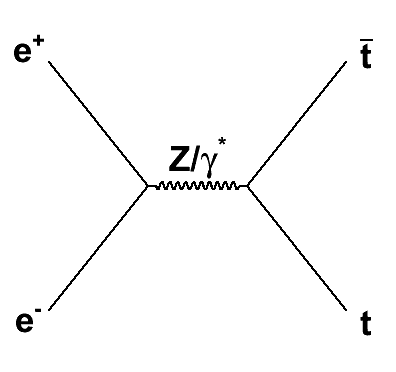
\includegraphics[width=0.35\linewidth]{Theory/fig/ttFeynmann}
\caption[Dominant top production mechanism at electron positron colliders]{Dominant top production mechanism at electron positron collider}
\label{fig:topFeynmann}
\end{figure}

\begin{equation}
\Gamma_{\mu}^{t\bar{t}X}(s,q,\bar{q})= ie\{ \gamma_{\mu}(F_{1V}^{X}(s)+ \gamma_{5}F_{1A}^{X}(s)) - \frac{\sigma_{\mu\nu}}{2m_t}(q+\bar{q})^{\nu}(iF_{2V}^{X}(s) + \gamma_{5}F_{2A}^{X}(s))\},
\end{equation}

where $X=\gamma /Z$, $q$ and $\bar{q}$ are the four momenta of the top and anti top, $s$ is $(q+\bar{q})^2$, $\gamma_\mu$ and $\gamma_\mu\gamma_5$ are the Dirac matrices corresponding to vector and axial-vector currents respectively, $\sigma_{\mu\nu}=\frac{i}{2}(\gamma_\mu \gamma_\nu -\gamma_\nu \gamma_\mu)$ allows for describing the scattering and $F$ are the electroweak form factors. Within the \ac{SM}, the only non-zero form factors at tree level are

\begin{equation}
F_{1V}^{\gamma}=\frac{2}{3},
\end{equation}

\begin{equation}
F_{1V}^{Z}=\frac{1}{4\sin\theta_{W}\cos\theta_{W}}(1-\frac{8}{3}\sin\theta_{W}),
\end{equation}

\begin{equation}
F_{1A}^{Z}=\frac{1}{4\sin\theta_{W}\cos\theta_{W}},
\end{equation}

where $\theta_W$ is the weak mixing angle. While the remaining form factors ($F_2$ and $F_{1A}^{\gamma}$) are predicted to be zero up to three-loop level in the \ac{SM}, several \ac{BSM} models predict they can gain a non-zero contribution at the one-loop level\cite{Abe:2001swa} making them a useful tool for probing the \ac{SM}. Combinations of these factors can be related to physical observables which can be measured at CLIC. The couplings of the bosons to quarks with left or right handed helicity can be expressed as

\begin{equation}
g_L^X = F_{1V}^{X} - F_{1A}^{X} ~~~~~~~~~~~ g_R^X = F_{1V}^{X} + F_{1A}^{X}
\end{equation}

The most directly observable experimental variables are the total cross section and the forward backward asymmetry (\afb). These are the measurements that are presented later within this thesis and will be discussed in more detail in Chapter \ref{chapter:topanalysis}. The forward backward asymmetry is of special interest as the measurement of the b quark forward-backward asymmetry at \ac{LEP}\cite{ABBIENDI200229} currently produces the largest tension with the \ac{SM}, $\mathcal{O}(3\sigma)$\cite{ALEPH:2005ab}, in electroweak fits. These variables are found to be dependent on the helicity of the incoming electrons \cite{Schmidt:1995mr} and so are more easily expressed in terms of the alternative form factors:

\begin{equation}
F_{ij}^{L} = -F_{ij}^{\gamma} +(\frac{-\frac{1}{2} +\sin\theta_W^2}{\sin\theta_W\cos\theta_W})(\frac{s}{s-m_Z^2}) -F_{ij}^{Z},
\end{equation}

\begin{equation}
F_{ij}^{R} = -F_{ij}^{\gamma} +(\frac{\sin\theta_W^2}{\sin\theta_W\cos\theta_W})(\frac{s}{s-m_Z^2}) -F_{ij}^{Z},
\end{equation}

where $L$,$R$ represent the polarization of the electron, $i$=1,2 and $j$=$V$,$A$. In this notation, for an electron polarization P, the total $ee\rightarrow Z/\gamma\rightarrow tt$ cross section and \afb can be expressed as:

\begin{equation}
\sigma_P = \frac{8\pi\alpha(s)^2}{s}\beta \{(1 + \frac{1}{2\gamma^2})(F_{1V}^P)^2 +(\beta F_{1A}^P)^2 +3F_{1V}^P F_{2V}^P + (1 + \frac{1}{2\gamma^2})(F_{2V}^P)^2\},
\end{equation}

\begin{equation}
\label{eq:afbFormFactors}
A_{FB}(P) = \mp \frac{12\pi\alpha(s)^2 \beta^2}{s}\frac{F_{1A}^P(F_{1V}^P +F_{2V}^P)}{\sigma_P},
\end{equation}

where $\alpha(s)$  is the electromagnetic coupling, $\gamma$ and $\beta$ are the Lorentz factor and speed of the top, and for \refeq{eq:afbFormFactors}, the $+$ and $-$ refer to the $P=R$ and $P=L$ cases respectively. A single measurement of the cross section and \afb alone would not allow the form factors to be determined because the system would be underconstrained. However, because the cross section and \afb vary with $\beta$, $\gamma$ and $P$, then by performing the measurement at multiple energies and making use of the fact that \ac{CLIC} can be operated with different beam polarizations, it becomes possible to extract all relevant couplings. An example of how \afb varies with the centre-of-mass of the collision, $\sqrt{s}$, for a fixed polarization is shown in \reffig{fig:AfbSDependence}, while the cross section dependence is shown in \reffig{Fig:SuperSym}. The only exceptions to this are the $F_{2A}^X$ factors which do not affect these two variables and so must be measured using alternative methods. 

\begin{figure}
  \centering
  \includegraphics[width=0.65\textwidth]{TopAnalysis/figures/asym-top.eps}
  \caption[Predicted forward backward asymmetry as a function of collision energy]{Predicted forward backward asymmetry as a function of collision energy\cite{Fleischer:2003kk}.}
  \label{fig:AfbSDependence}
\end{figure}

\begin{figure}
\centering
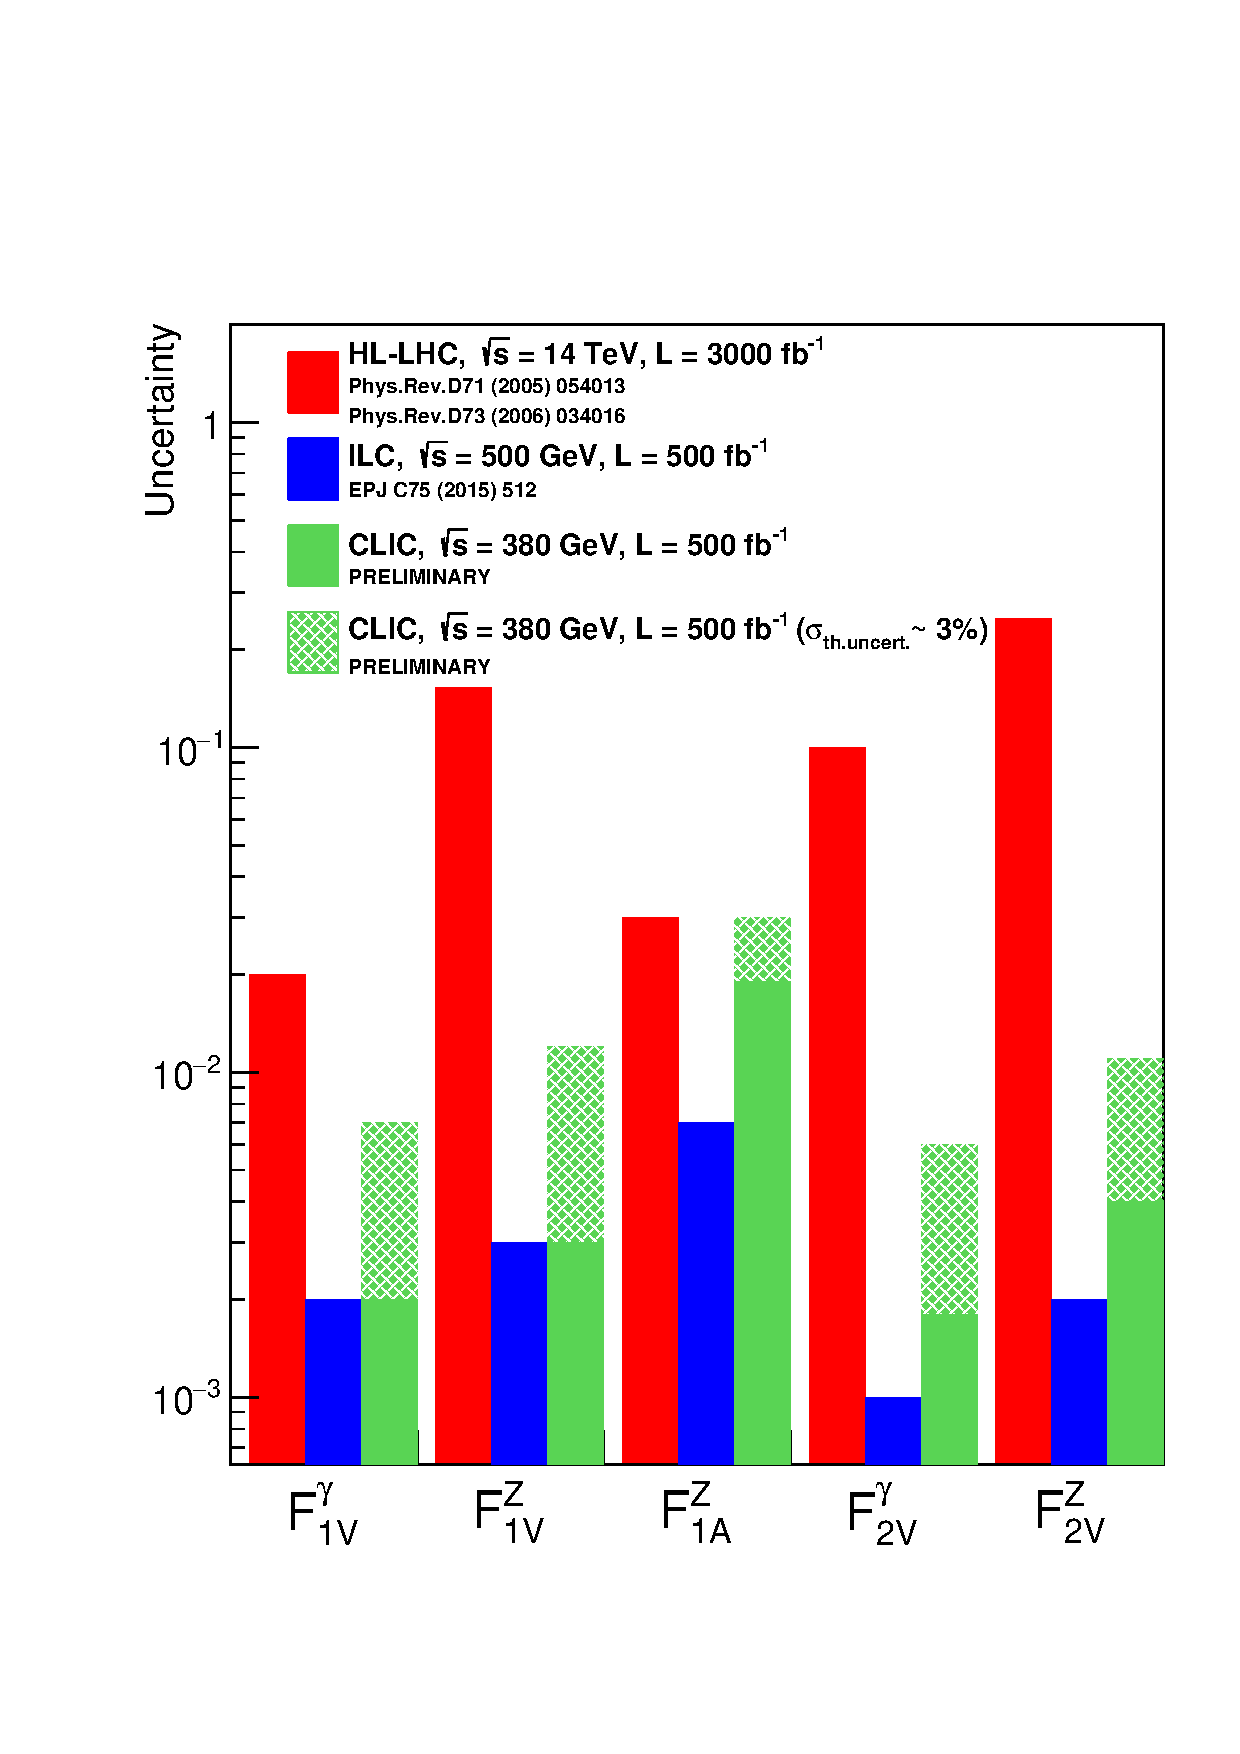
\includegraphics[width=0.65\linewidth]{Theory/fig/FormFactorsTopCLIC380.pdf}
\caption[Expected precision on CP conserving electroweak form factors at future colliders]{Expected precision on CP conserving electroweak form factors at future colliders \cite{CLIC:2016zwp}}
\label{fig:CPConserving}
\end{figure}

The predicted uncertainty with which the couplings are expected to be measured at \ac{CLIC} based on generator level studies, as well as the equivalent results for \ac{ILC} and \ac{HL-LHC}, is shown in \reffig{fig:CPConserving}. The expected precision from performing these measurements at a lepton collider is an order of magnitude better than that expected from hadron colliders. Overall there will be more tops produced in a hadron collider, however the production mechanisms are often more complicated making it harder to extract the couplings. As a result the form factors will usually be extracted from ttZ and tt$\gamma$ final states rather than s-channel production\cite{Baur:2005wi} which makes them harder to relate to observables such as \afb. It is also harder to identify tops (which typically decay to at least one jet) in an environment that contains \ac{QCD} jets from beam remnants compared to at lepton colliders where there is minimal \ac{QCD} background within an event.
